\documentclass[11pt,english]{article}

%%%%%%%%%%%%%%%%%%%%%%%%%%%%%%%%%%%%%%%%%%%%%%%%%%%%%%%%%%%
% Packages
%%%%%%%%%%%%%%%%%%%%%%%%%%%%%%%%%%%%%%%%%%%%%%%%%%%%%%%%%%%

% paper size & margins
\usepackage{fullpage}
\usepackage[showframe=false,margin=1in]{geometry}
\parindent=0pt

% font management
\usepackage{relsize}
\usepackage[T1]{fontenc} % for properly hyphenating words with accented chars
\usepackage[latin1]{inputenc}
\usepackage{babel}

% math
\usepackage{amsmath}
\usepackage{amsthm}
\usepackage{amssymb}
\usepackage{textcomp}
\usepackage{stmaryrd}
\usepackage{upgreek}
\usepackage{bm}
\usepackage[linesnumbered,ruled,vlined]{algorithm2e}

% assorted
\usepackage{url}
\usepackage{breakurl}
\usepackage{xspace}
\usepackage{comment}
\usepackage{color}
\usepackage{xcolor}
\usepackage{afterpage}
\usepackage{graphicx}
\usepackage{hyperref}
\usepackage{pdfpages}
\usepackage{subcaption}
\usepackage{multirow}
\usepackage{placeins}
\usepackage{listings}

%%%%%%%%%%%%%%%%%%%%%%%%%%%%%%%%%%%%%%%%%%%%%%%%%%%%%%%%%%%
% Shortcuts
%%%%%%%%%%%%%%%%%%%%%%%%%%%%%%%%%%%%%%%%%%%%%%%%%%%%%%%%%%%
\newcommand{\hide}[1]{}

\usepackage{environ}
\usepackage{xparse}

\ExplSyntaxOn
\NewEnviron{bmatrixT}
{
\marine_transpose:V \BODY
}

\int_new:N \l_marine_transpose_row_int
\int_new:N \l_marine_transpose_col_int
\seq_new:N \l_marine_transpose_rows_seq
\seq_new:N \l_marine_transpose_arow_seq
\prop_new:N \l_marine_transpose_matrix_prop
\tl_new:N \l_marine_transpose_last_tl
\tl_new:N \l_marine_transpose_body_tl

\cs_new_protected:Nn \marine_transpose:n
{
\seq_set_split:Nnn \l_marine_transpose_rows_seq { \\ } { #1 }
\int_zero:N \l_marine_transpose_row_int
\prop_clear:N \l_marine_transpose_matrix_prop
\seq_map_inline:Nn \l_marine_transpose_rows_seq
{
\int_incr:N \l_marine_transpose_row_int
\int_zero:N \l_marine_transpose_col_int
\seq_set_split:Nnn \l_marine_transpose_arow_seq { & } { ##1 }
\seq_map_inline:Nn \l_marine_transpose_arow_seq
{
\int_incr:N \l_marine_transpose_col_int
\prop_put:Nxn \l_marine_transpose_matrix_prop
{
\int_to_arabic:n { \l_marine_transpose_row_int }
,
\int_to_arabic:n { \l_marine_transpose_col_int }
}
{ ####1 }
}
}
\tl_clear:N \l_marine_transpose_body_tl
\int_step_inline:nnnn { 1 } { 1 } { \l_marine_transpose_col_int }
{
\int_step_inline:nnnn { 1 } { 1 } { \l_marine_transpose_row_int }
{
\tl_put_right:Nx \l_marine_transpose_body_tl
{
\prop_item:Nn \l_marine_transpose_matrix_prop { ####1,##1 }
\int_compare:nF { ####1 = \l_marine_transpose_row_int } { & }
}
}
\tl_put_right:Nn \l_marine_transpose_body_tl { \\ }
}
\begin{bmatrix}
    \l_marine_transpose_body_tl
\end{bmatrix}
}
\cs_generate_variant:Nn \marine_transpose:n { V }
\cs_generate_variant:Nn \prop_put:Nnn { Nx }
\ExplSyntaxOff


\definecolor{codewhite}{rgb}{0.95,0.95,0.95}
\definecolor{codegreen}{rgb}{0,0.6,0}
\definecolor{codegray}{rgb}{0.5,0.5,0.5}
\definecolor{codepurple}{rgb}{0.58,0,0.82}
\definecolor{backcolour}{rgb}{0.1,0.1,0.1}

\lstdefinestyle{mystyle}{
    backgroundcolor=\color{backcolour},
    commentstyle=\color{codegreen},
    keywordstyle=\color{orange},
    numberstyle=\tiny\color{codegray},
    stringstyle=\color{codepurple},
    basicstyle=\ttfamily\scriptsize\color{codewhite},
    breakatwhitespace=false,
    breaklines=true,
    captionpos=b,
    keepspaces=true,
    numbers=left,
    numbersep=5pt,
    showspaces=false,
    showstringspaces=false,
    showtabs=false,
    tabsize=2
}

\lstset{style=mystyle}


%%%%%%%%%%%%%%%%%%%%%%%%%%%%%%%%%%%%%%%%%%%%%%%%%%%%%%%%%%%
% Title / Author
%%%%%%%%%%%%%%%%%%%%%%%%%%%%%%%%%%%%%%%%%%%%%%%%%%%%%%%%%%%
\begin{document}

    \title{CS7643: Deep Learning \\
    Fall 2019\\ HW3 Solutions}
    \author{Nicolas \textsc{Six}}
    \maketitle


    %%%%%%%%%%%%%%%%%%%%%%%%%%%%%%%%%%%%%%%%%%%%%%%%%%%%%%%%%%%
    % Body
    %%%%%%%%%%%%%%%%%%%%%%%%%%%%%%%%%%%%%%%%%%%%%%%%%%%%%%%%%%%

    \section{Recurrent Neural Network}
    \subsection{Vanilla RNN for parity function} \label{q1.1}
    
If this function has a minimum, it has to be when its partial derivative regarding to $\vec{w}$ is null.
In addition, as the this function is convex, so admit only one point where $\vec{w}$ is null, and so only one extrema.
As this function is clearly unbounded from above this extrema is the global minimum.

\begin{align*}
    \frac{\partial \left( f\left( \vec{w^{(t)}} \right) +
                           \left< \vec{w} - \vec{w^{(t)}}, \nabla f\left( \vec{w^{(t)}} \right) \right>
                           + \frac{\lambda}{2} \left\| \vec{w} - \vec{w^{(t)}} \right\|^2 \right)
    }{
        \partial \vec{w}
    }
    &= 0 \\
    \Leftrightarrow
    \frac{\partial \left(
                           \left< \vec{w}, \nabla f\left( \vec{w^{(t)}} \right) \right> \right) }
    {\partial \vec{w}} +
    \frac{\partial \left( \frac{\lambda}{2} \left< \vec{w} - \vec{w^{(t)}}, \vec{w} - \vec{w^{(t)}} \right> \right) }
    {\partial \vec{w}}
    &= 0 \\
    \Leftrightarrow
    \left< \frac{\partial\vec{w}}{\partial\vec{w}}, \nabla f\left( \vec{w^{(t)}} \right) \right> +
    \lambda \left< \frac{\partial\vec{w}}{\partial\vec{w}}, \vec{w} - \vec{w^{(t)}} \right>
    &= 0 \\
    \Leftrightarrow
    \left< \frac{\partial\vec{w}}{\partial\vec{w}}, \nabla f\left( \vec{w^{(t)}} \right) + \lambda \left( \vec{w} - \vec{w^{(t)}} \right) \right>
    &= 0 \\
    \Leftrightarrow
    \nabla f\left( \vec{w^{(t)}} \right) + \lambda \left( \vec{w} - \vec{w^{(t)}} \right)
    &= \vec{0} \\
    \Leftrightarrow
    \vec{w}
    &= \vec{w^{(t)}} - \frac{1}{\lambda} \nabla f\left( \vec{w^{(t)}} \right) \\
\end{align*}

In conclusion we get the following:

\begin{align*}
    \vec{w^*} &= \vec{w^{(t)}} - \frac{1}{\lambda} \nabla f\left( \vec{w^{(t)}} \right) \\
    \eta &= \frac{1}{\lambda}
\end{align*}

This show us that under our current set of assumption, the gradient descent is leading us the the optimal solution.
    \clearpage
    \pagebreak
    \subsection{LSTM for parity function} \label{q1.2}
    The optimal policy is $("go","go")$.
Lets name this policy $\pi^*$.
Now we can compute the value of each state following this policy.

\begin{align*}
    V^*(S_2) &= r(S_2, "go") \\
    &= 3
    V^*(S_1) &= r(S_1, "go") + \gamma V^*(S_2) \\
    &= -2 + 3 \gamma
\end{align*}




    \pagebreak
    \subsection{When to stop in beam search?} \label{q1.3}
    

\begin{align*}
    V^0 &= [0,0] \\
    V^1 &= [-1,3] \\
    V^2 &= [1,3] \\
    V^3 &= [1,3] \\
    V^* &= [1,3]
\end{align*}


    \pagebreak
    \subsection{Exploding Gradients} \label{q1.4}
    
\paragraph{}
For this question we will suppose that $W$ is a diagonalizable matrix, which is implied by the fact that it's
eigenvalues are given in the subject.

With that in mind, we know that it exist a matrix $Q$ such as:

\[
    W^T = Q D Q^{-1}
\]

\paragraph{}
With $D$ being a diagonal matrix with tha eigenvalues of $W$ on the diagonal (and $Q$ the eigenvectors).

\paragraph{}
Using this we can easily rewrite the given equation as:
\begin{align*}
    h_t &= W^T h_{t-1} \\
        &= Q D Q^{-1} h_{t-1} \\
    h_t &= Q D^t Q^{-1} h_{0}
\end{align*}

\paragraph{}
It is trivial that raising a diagonal matrix to a power $t$ is equivalent to raise each of it's diagonal element to the
power $t$.
So depending on the value of the eigenvalues, raising the matrix $D$ to a high power will make the diagonal element
tend to zero (vanish) if they are smaller than one (in absolute value).
If they are bigger than one (in absolute value) they will diverge to infinity.
Or change signs / stay the same of they are $1$ or $-1$.

\paragraph{}
This matrix is then used to compute the output, $h_t$, but also in the backward pass to propagate the gradient.
Especially for the first inputs.
So the gradient could be multiplied by values that are either too big (exploding) or too small (vanishing).



    \pagebreak
    \section{Coding: Sequence models for image captioning}
    \subsection{RNN Captioning}
    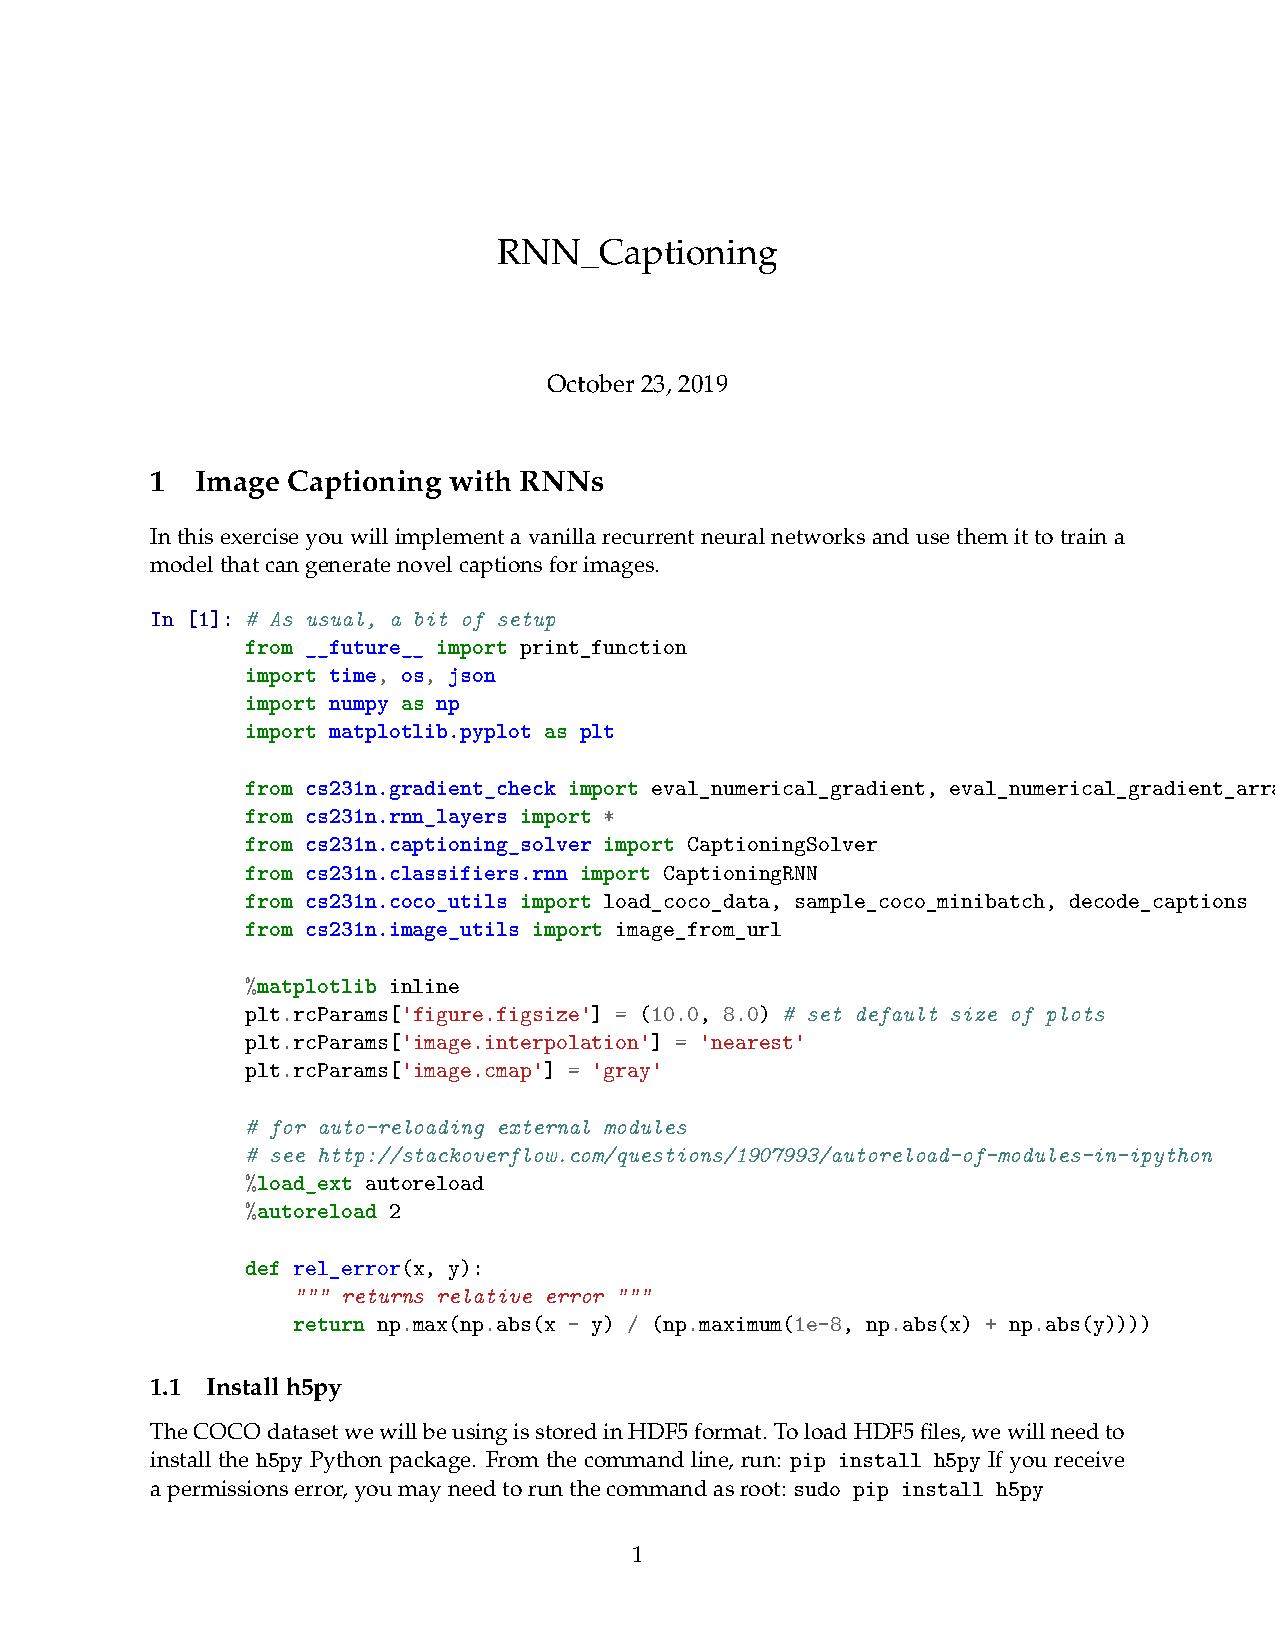
\includepdf[pages=-]{../code/RNN_Captioning.pdf}

    \subsection{LSTM Captioning}
    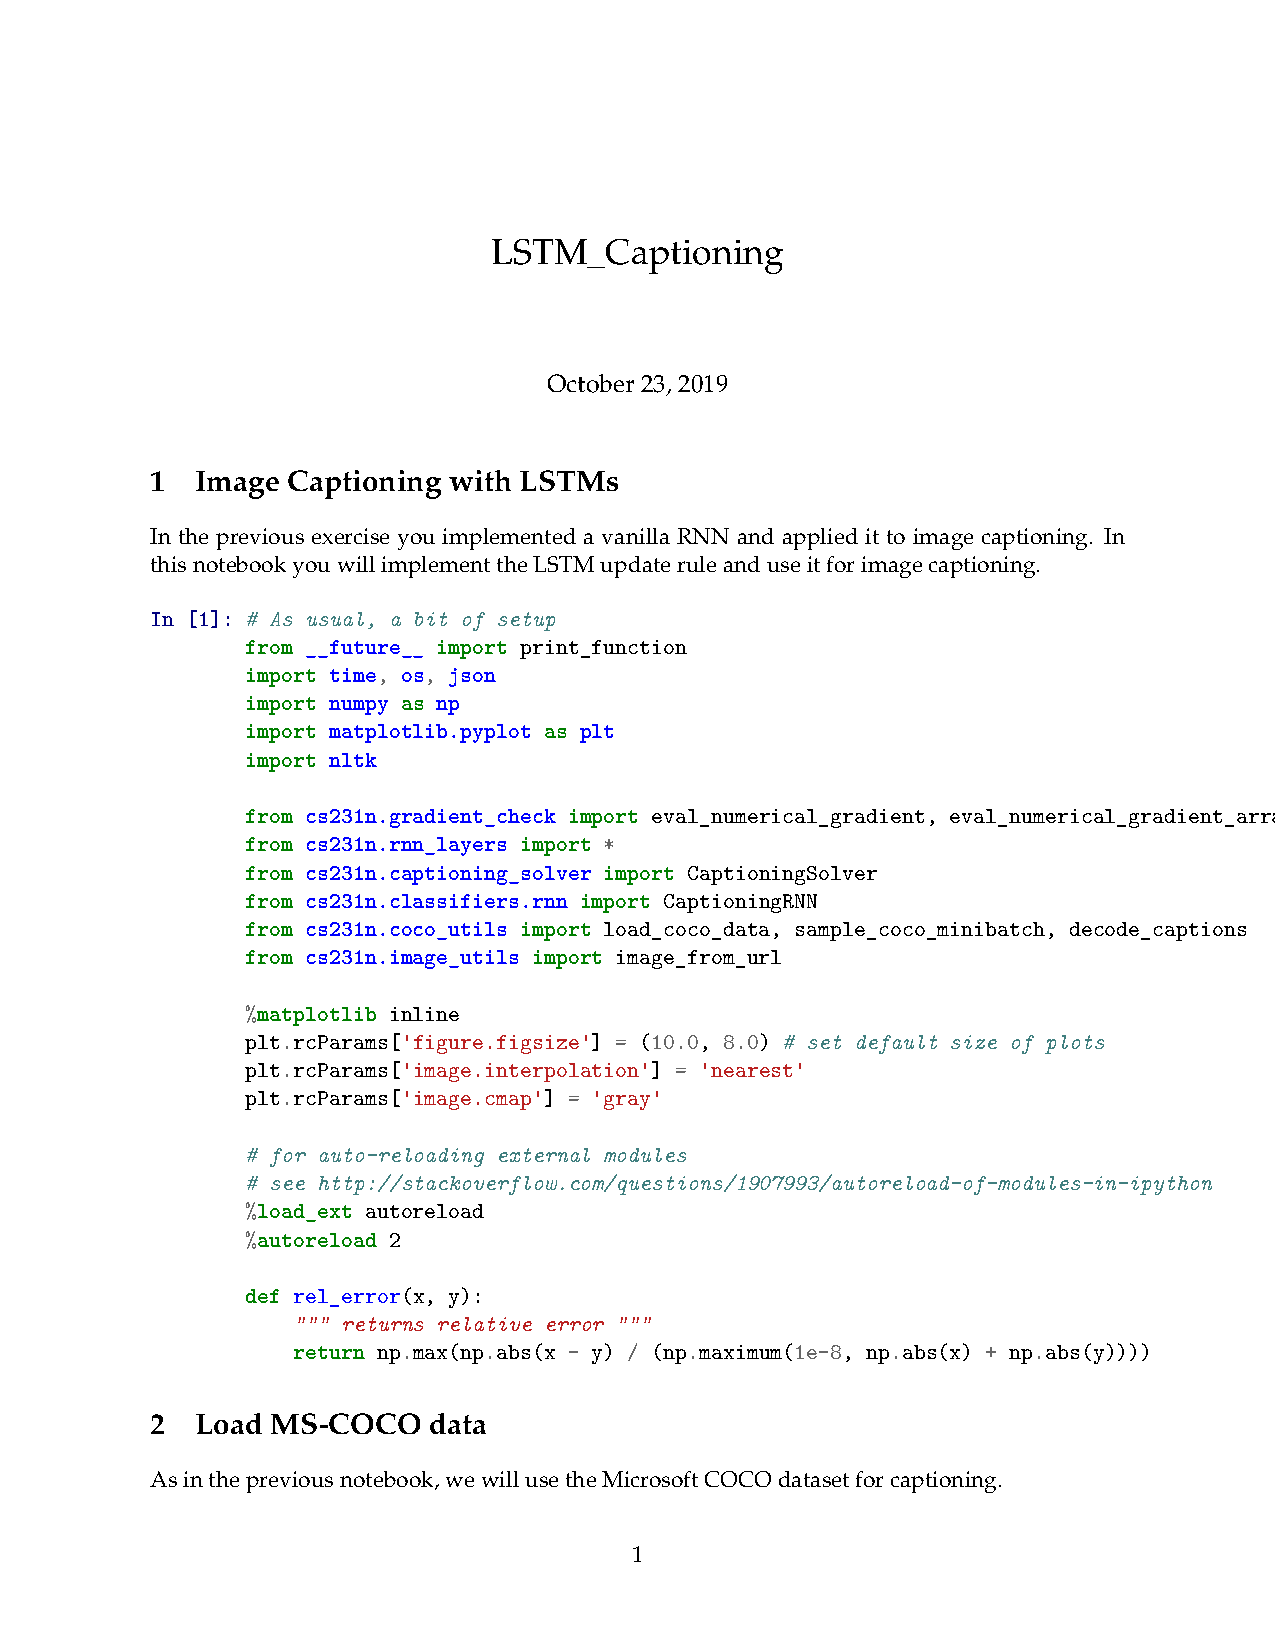
\includepdf[pages=-]{../code/LSTM_Captioning.pdf}

    \subsection{Transformer Classification}
    \subsubsection{Ipython notebook}
    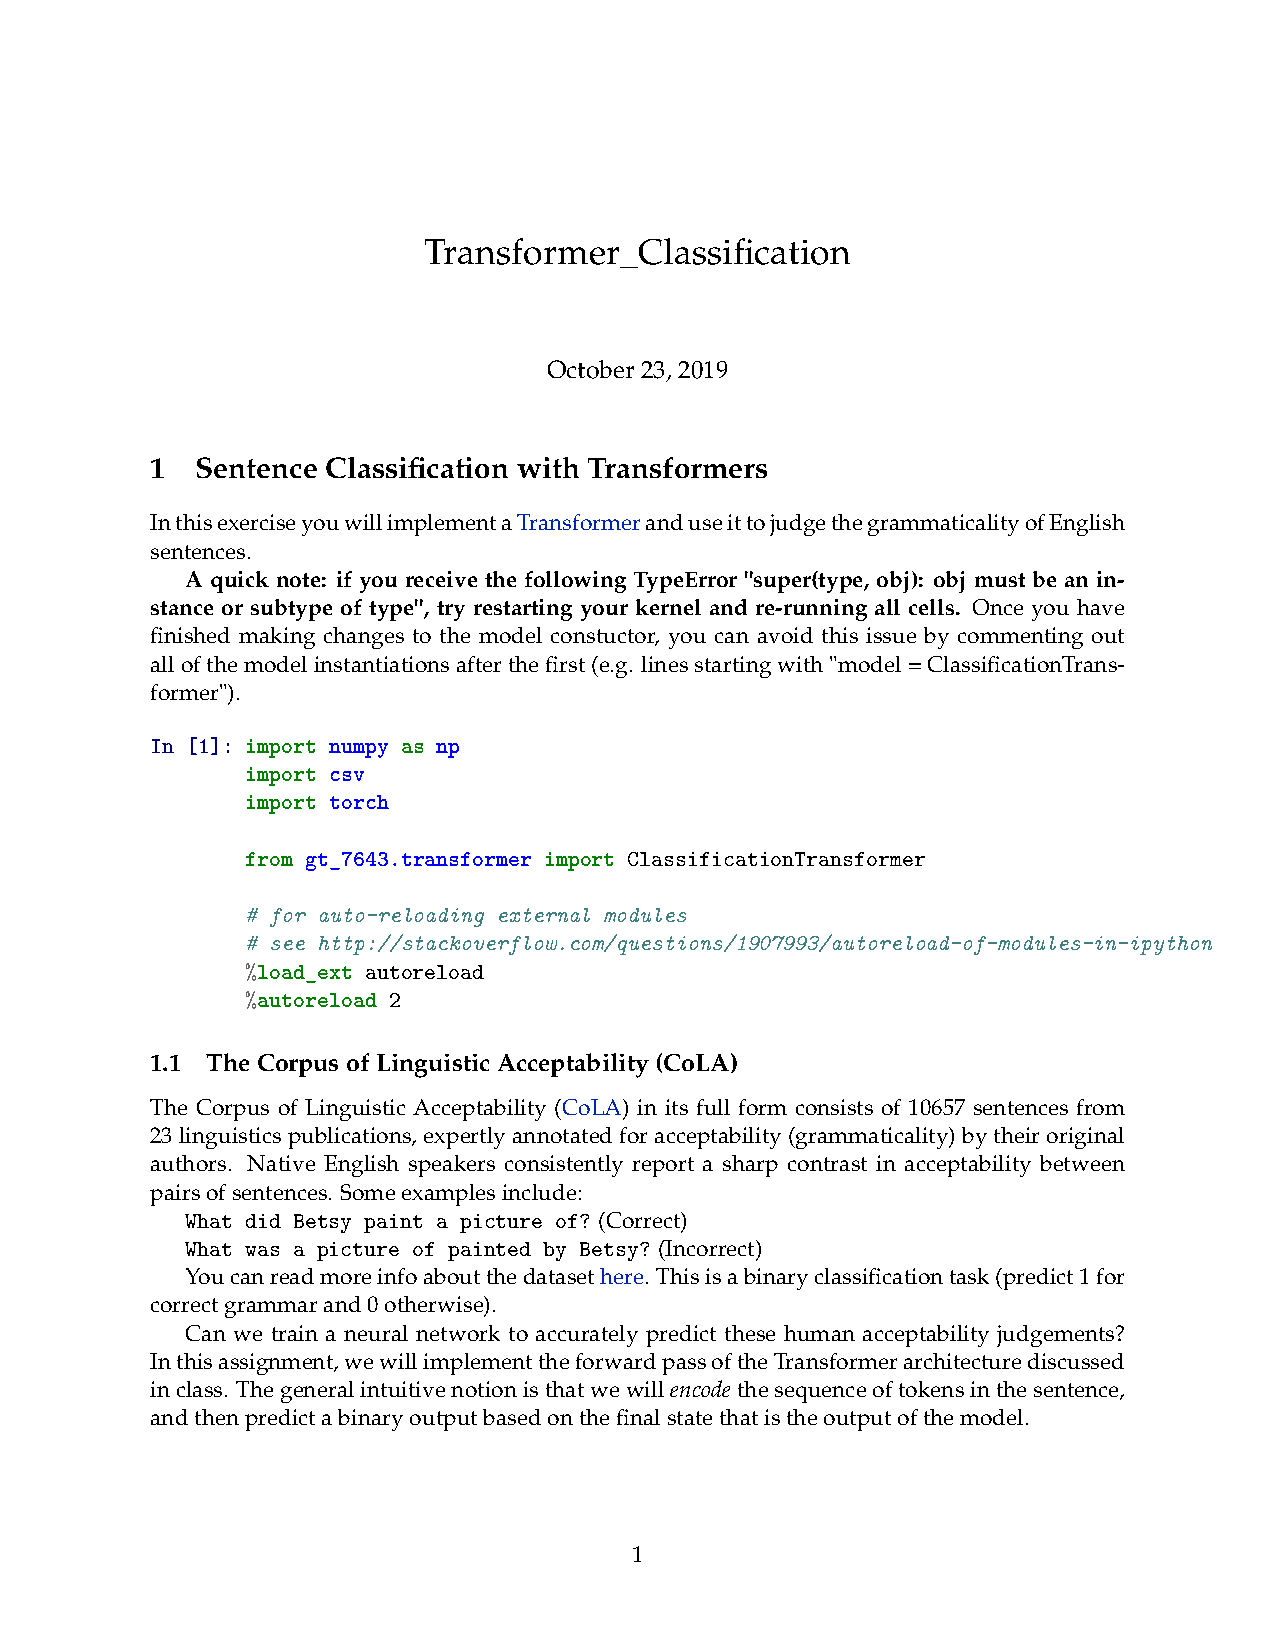
\includepdf[pages=-]{../code/Transformer_Classification.pdf}

    \subsubsection{Python code}
    \lstinputlisting[language=Python]{../code/gt_7643/transformer.py}

\end{document}
